\chapter{Implementation Frontend}

This chapter explains the implementation of the frontend of the compiler. First the additional technologies that are used in the development of the frontend are listed. Then the AST and symboltable are explained. In the following section the ANTLR grammar is shown. Based on this grammar three implementations for the AST transformation are explained: Visitor-pattern, listener-pattern and via an attributed grammar. 

\section{Used Technologies}

In this section the additional technologies used for the development of the frontend are explained. This includes chosen the programming language and the additional libraries used.

\subsection{Kotlin}

For the implementation the programming language Kotlin is chosen. Kotlin can be compiled to bytecode, which makes it possible to use Java libraries in Kotlin code. Kotlin has advantages over Java in some aspects. For example, null safety\footnote{https://kotlinlang.org/docs/null-safety.html} is implemented into the language via explicit nullability within it's type system. This requires the caller of a field to explicitly handle nullable fields and thus reduces the risk of a null reference exception. 

\subsection{AspectJ}

The compiler frontend utilizes AspectJ in it's handling of semantic errors. AspectJ is a library that enables aspect oriented programming in Java. Aspect oriented programming makes it possible to handle cross-cutting concerns in a central place without having to modify code in other areas. It can be used for compile time and runtime weaving of cross-cutting concerns. In the compiler frontend, runtime weaving using annotations is used.  

\subsection{ANTLR Preview Plugin}

During development with the JetBrains IntelliJ IDE, the ANTLR preview plugin\footnote{https://plugins.jetbrains.com/plugin/7358-antlr-v4} is used. The plugin developed by the ANTLR creator Terrance Parr, offers various features that enhance the process of creating and working with ANTLR. When developing an ANTLR grammar, syntax highlighting and checking for syntactic and semantic errors is provided. The included navigation window inside the IDE further enables testing of the grammar, without having to generate the combined lexer and parser manually first. To generate the combined lexer and parser the plugin includes a tool window which includes common configuration settings.

\section{ANTLR Grammar}
\label{cha:ANTLRGrammar}

The ANTLR grammar is based on the MiniC++ grammar in EBNF-form. This grammar is transformed into the ANTLR grammar syntax. ANTLR grammars are stored inside \texttt{.g4} files. Each rule inside the grammar is delimited by a semicolon. 

\subsection{Header Section}

At the top of the grammar file, the name of the grammar is specified. In this case \texttt{minicpp}. In this section options can also be specified, like the implementation language of the lexer and parser or the package/namespace of the generated code. These and other options can also be specified via command line options during the generation. In this case the necessary options are specified in the tool window of the ANTLR preview plugin. 

%if in need add picture of tool window

\subsection{Terminal Classes and Comments}

The grammar contains three terminal classes shown in listing \ref{lst:ANTLRMiniCppTermClass}. The \texttt{IDENT} terminal class is used for all identifiers and requires them to start with a letter followed by an arbitrary number of letters and digits. For integer number the \texttt{INT} terminal class specifies a sequence of one or more digits. Signs are handled in the parser rules. Strings are defined as a sequence of characters starting and ending with double quotes. All characters except the special characters for line end are allowed. The comment and whitespace handling is performed by the \texttt{WS}, \verb|LINE_COMMENT| and \verb|BLOCK_COMMENT| lexical rules. These are special rules that when matched tell the parser to skip them and therefore not include them in the syntax tree. 

\begin{AntlrCode}[float,numbers=none,caption=Terminal classes of the MiniC++ ANTLR grammar., label=lst:ANTLRMiniCppTermClass]
IDENT:          [a-zA-Z_][a-zA-Z_0-9]*;
INT:            [0-9]+;
STRING:         '"' (~[\r\n"] | '""')* '"';
WS:             [ \t\n\r]+ -> skip;
LINE_COMMENT:   '//' ~[\r\n]* -> skip;
BLOCK_COMMENT:  '/*' .*? '*/' -> skip;
\end{AntlrCode}


\subsection{Root}

The top rules of the grammar are shown in listing \ref{lst:ANTLRMiniCppTop}. The root rule \texttt{miniCpp} contains zero or more elements of the rule \texttt{miniCppEntry} followed by the lexical rule \texttt{EOF}. \texttt{EOF} is a default lexical rule provided by ANTLR signaling the end of the file. \texttt{miniCppEntry} defines the elements that can be used at the top level of the miniC\verb|++| source file. These are variable and constant definitions and function declarations and definitions. \texttt{SEM} is the lexical rule defining a semicolon. 

\begin{AntlrCode}[float,numbers=none,caption=Top rules of the MiniC++ ANTLR grammar., label=lst:ANTLRMiniCppTop]
miniCpp:     (miniCppEntry)* EOF;
miniCppEntry:     constDef
                | varDef
                | funcDecl
                | funcDef
                | SEM
                ;
\end{AntlrCode}



\subsection{Variables and Constants}

Listing \ref{lst:ANTLRMiniCppVarConstDef} shows the parser rules variable and constant definitions. Both definitions can have multiple entries, which are separated by a comma. In the case of a constant definition entry, the initialization value is required. For a variable this is optional. The \texttt{STAR} optional lexical rule classifies a field as an array if present. The \texttt{initOption} parser rule consists of three production alternatives specifying the possible initialization values. 

\begin{AntlrCode}[float,numbers=none,caption=Variable and constant defintions of the MiniC++ ANTLR grammar., label=lst:ANTLRMiniCppVarConstDef]
constDef:        CONST type constDefEntry (COMMA constDefEntry)* SEM ;
constDefEntry:   IDENT init ;

varDef:          type varDefEntry (COMMA varDefEntry)* SEM ;
varDefEntry:     STAR? IDENT (init)? ;

init:            EQUAL  initOption ;
initOption:      BOOLEAN      #BooleanInit
               | NULLPTR      #NullptrInit
               | (SIGN)? INT  #IntInit
               ;
\end{AntlrCode}

\subsection{Function Declaration and Definition}

The rules for a function declaration and definition are shown in listing \ref{lst:ANTLRMiniCppFuncDeclDef}. In MiniC\verb|++| to call a function there must be at least a declaration of the function further ahead in the source code. Function declarations and definitions both start with the function head that consists of the return type, identifier and an optional parameter list. In the case of a function definition, the function head is followed the \texttt{block} rule, which contains the method's body. 

The parameter list can consist either of a single entry, the \texttt{void} type, or of one or more actual input parameters. Each parameter specified by the \texttt{formParListEntry} rule, consists of a type, an optional star and brackets indicating an array followed by the identifier of the parameter.


\begin{AntlrCode}[float,numbers=none,caption=Function declaration and defintion of the MiniC++ ANTLR grammar., label=lst:ANTLRMiniCppFuncDeclDef]
funcDecl:         funcHead SEM;
funcDef:          funcHead block;
funcHead:         type STAR? IDENT LPAREN formParList? RPAREN;
formParList:      (     VOID
                  |     formParListEntry (COMMA formParListEntry)*
                  );
formParListEntry: type STAR? IDENT (BRACKETS)?;
\end{AntlrCode}

\subsection{Statements}

The parser rule defining a statement is shown in listing \ref{lst:ANTLRMiniCppStatAlt}. The statement rules serves as a container for all concrete statement types. For example, the \texttt{ifStat} rule can be seen in listing \ref{lst:ANTLRMiniCppStatIf}. It consists of the \texttt{if} keyword followed by the condition in parentheses and a statement which should be executed if the condition is met. Optionally an else statement can be specified. This rule does not suffer from the \textit{dangling else} problem. In such cases ANTLR resolves the ambiguity by always choosing the first successful production. 

\begin{AntlrCode}[float,numbers=none,caption=Statement rule and it's production alternatives of the MiniC++ ANTLR grammar., label=lst:ANTLRMiniCppStatAlt]
stat:  ( emptyStat  | breakStat
       | blockStat  | exprStat
       | ifStat     | whileStat
       | inputStat  | outputStat
       | deleteStat | returnStat
       );
\end{AntlrCode}

\begin{AntlrCode}[float,numbers=none,caption=If Statement rule  of the MiniC++ ANTLR grammar., label=lst:ANTLRMiniCppStatIf]
ifStat:      'if' LPAREN expr RPAREN stat elseStat?;
elseStat:    'else' stat;
\end{AntlrCode}



\subsection{Expressions}

Part of the grammar for expressions is shown in listing \ref{lst:ANTLRMiniCppExprBool}. At the top of every expression is an \texttt{orExpr} followed by zero or more \texttt{exprEntry} elements. In case an \texttt{exprEntry} is present, the expression performs one or mor assignments. Each \texttt{exprEntry} consists of an assignment operator signalizing the type of assignment, and an \texttt{orExpr} that provides the value to be assigned. The \verb|orExpr| and \verb|andExpr| rules implement their respective boolean operators. The \verb|relExpr| rule consists of a \verb|simpleExpr| and zero or more \verb|relExprEntry| elements. The \verb|relExprEntry| rule handles relative expressions with the \verb|relExprOperator| rule, which contains the relative operators like greater or less than. The \verb|simpleExpr| rule begins with an optional sign that is relevant for integer values, followed by a term and zero or more \verb|simpleExprEntry| elements. The \verb|simpleExprEntry| rule consists of a sign followed by a term. The precedence rules for arithmetic operations are realized inside the grammar.



\begin{AntlrCode}[float,numbers=none,caption=Expression rules for assignment and boolean operations of the MiniC++ ANTLR grammar., label=lst:ANTLRMiniCppExprBool]
expr:                 orExpr (exprEntry)*;
exprEntry:            exprAssign orExpr;
exprAssign:           EQUAL      #EqualAssign
                    | ADD_ASSIGN #AddAssign
                    | SUB_ASSIGN #SubAssign
                    | MUL_ASSIGN #MulAssign
                    | DIV_ASSIGN #DivAssign
                    | MOD_ASSIGN #ModAssign
                    ;
orExpr:             andExpr ( '||' andExpr )*;
andExpr:            relExpr ( '&&' relExpr )*;
relExpr:            simpleExpr
                    ( relExprEntry )*;
relExprEntry:       relOperator simpleExpr;
simpleExpr:         (SIGN)?
                    term ( simpleExprEntry )*;
simpleExprEntry:    SIGN term;
\end{AntlrCode}

The rules for terms and factors are shown in listing \ref{lst:ANTLRMiniCppExprTermFact}. A term consists of a fact, which contains an optional negation making it a \verb|notFact|, followed by zero or more \verb|termEntry| elements. The \verb|termEntry| rule realizes multiplication, division and modulo operations via the \verb|termOperator| rule. The \verb|fact| rule contains six possible productions. Three types of value literals can be used as a factor: integer, boolean or null-pointer. Another option is the array initialization, defined by the \verb|#NewArrayFact| alternative. The \verb|#ExprFact| alternative allows for precedence using an expression contained in parentheses. To read the value of a variable or array, or call a function the \verb|#CallFact| alternative using the \verb|callFactEntry| rule is used. The \verb|callFactEntry| rule contains an optional increment/decrement at the beginning and end of the rule. Each \verb|INC_DEC| element has a named alias so that in the syntax tree it can be easily checked which element is null. Via the \verb|IDENT| terminal class the name of the variable or array to read can be specified. If \verb|callFactEntryOperation| is not null, then either a function call or array access is performed. Depending on the type of function that is called, parameters may be necessary. The \verb|#ActParListFactOperation| alternative allows for parameters via the optional \verb|actParList| rule. This rule consists of one or more expressions, that make up the parameters.     

\begin{AntlrCode}[float,numbers=none,caption=Expression rules for terms and factors of the MiniC++ ANTLR grammar., label=lst:ANTLRMiniCppExprTermFact]
term:             notFact (termEntry)*;
termEntry:        termOperator notFact;
termOperator:     STAR #StarOperator
                | DIV #DivOperator
                | MOD #ModOperator;
notFact:          NOT? fact;
fact:             BOOLEAN #BooleanFact
                | NULLPTR #NullptrFact
                | INT     #IntFact
                | callFactEntry         #CallFact
                | NEW type LBRACK expr RBRACK #NewArrayFact
                | LPAREN expr RPAREN          #ExprFact
                ;
callFactEntry:    preIncDec=INC_DEC?
                  IDENT
                  callFactEntryOperation?
                  postIncDec=INC_DEC?
                  ;
callFactEntryOperation:
      ( LBRACK expr    RBRACK)          #ExprFactOperation
    | ( LPAREN (actParList)?    RPAREN) #ActParListFactOperation
    ;
actParList:       expr (COMMA expr)*;
\end{AntlrCode}

\section{Abstract Syntax Tree (AST)}

The syntax tree created by ANTLR contains information that is not necessary for the later stages of the compiler. For this reason an abstract syntax tree (AST) is generated from the syntax tree. 

For the implementation of the AST nodes Kotlin \textit{data classes} are used primarily. A Kotlin \texttt{data class} provides implementations for common methods like \texttt{equals} and \verb|hashCode|. The method implementations are generated from the primary constructor of the data class. For leaf nodes which always contain the same information, e.g. the \verb|VOID| of the \verb|formParList| rule, Kotlin's \verb|data object| construct is used. A \verb|data object| is a singleton built into the language itself. In case a rule has more than one possible production, interfaces are used. Specifically Kotlin provides \textit{sealed} interfaces. With sealed interfaces, all classes that implement the interface are known at compile time. This allows for exhaustive pattern matching using the \verb|when| expression. 

The root class of the AST is \verb|MiniCpp|. It serves as a container for all classes that implement the \verb|MiniCppEntry| interface. The implementation classes are shown in figure \ref{fig:MiniCppEntriesDiag}. \verb|Sem| is a \verb|data object| since it encodes the same information every time it is used. \verb|ConstDef| and \verb|VarDef| both contain a list of entries, which store the information of the variables. For type management the AST uses the \verb|ExprType| enum shown in figure \ref{lst:ListExprType}. This enum contains all possible data types that can be used in MiniC\verb|++|. It further includes a descriptor which is used in the backend of the compiler during the bytecode generation. The \verb|FuncDef| and \verb|FuncDecl| classes store the information about the function's signature in the \verb|FuncHead| class. The  \verb|FuncDef| class further includes a field which contains the actual body of the function in the form of the \texttt{Block} class. A block consists of many block entries. Each block entry is a class that implements the \verb|BlockEntry| sealed interface. These are \verb|VarDef|, \verb|ConstDef| and the sealed interface \verb|Stat|. All concrete statement types like a while statement inherit from the \verb|Stat| interface. 

The AST nodes for expressions follow a similar pattern. The hierarchy is similar to the structure defined in the grammar. For the representation of a factor the \verb|Fact| interface is used. The classes that implement the \verb|Fact| interface are shown in figure \ref{fig:FactDiag}. The \verb|DataType| interface is responsible for handling literals. Each of its implementation classes is responsible for handling one type of literal, e.g. the \verb|IntType| for integer literals. For the instantiation of an array the \verb|NewArrayTypeFact| class provides the required information. The \verb|type| field stores the data type of the array. The expression provides an integer value which serves as the length of the array. For nesting of expressions the \verb|ExprFact| class is used. For reading a variable or array value and calling a function the \verb|ActionFact| class is used. The \verb|prefix| and \verb|suffix| fields are responsible for the optional increment/decrement operator. In case the \verb|actionOp| field is null, the identifier is the name of a variable whose value should be read. \verb|ActionOperation| is again an interface which is implemented by the \verb|ArrayAccessOperation| and \verb|CallOperation|. The \verb|ArrayAccessOperation| contains an expression which provides the index for the array access. The \verb|CallOperation| consists of the actual parameter list for the function call which is a list of expressions.

\begin{figure}[]
       \centering
       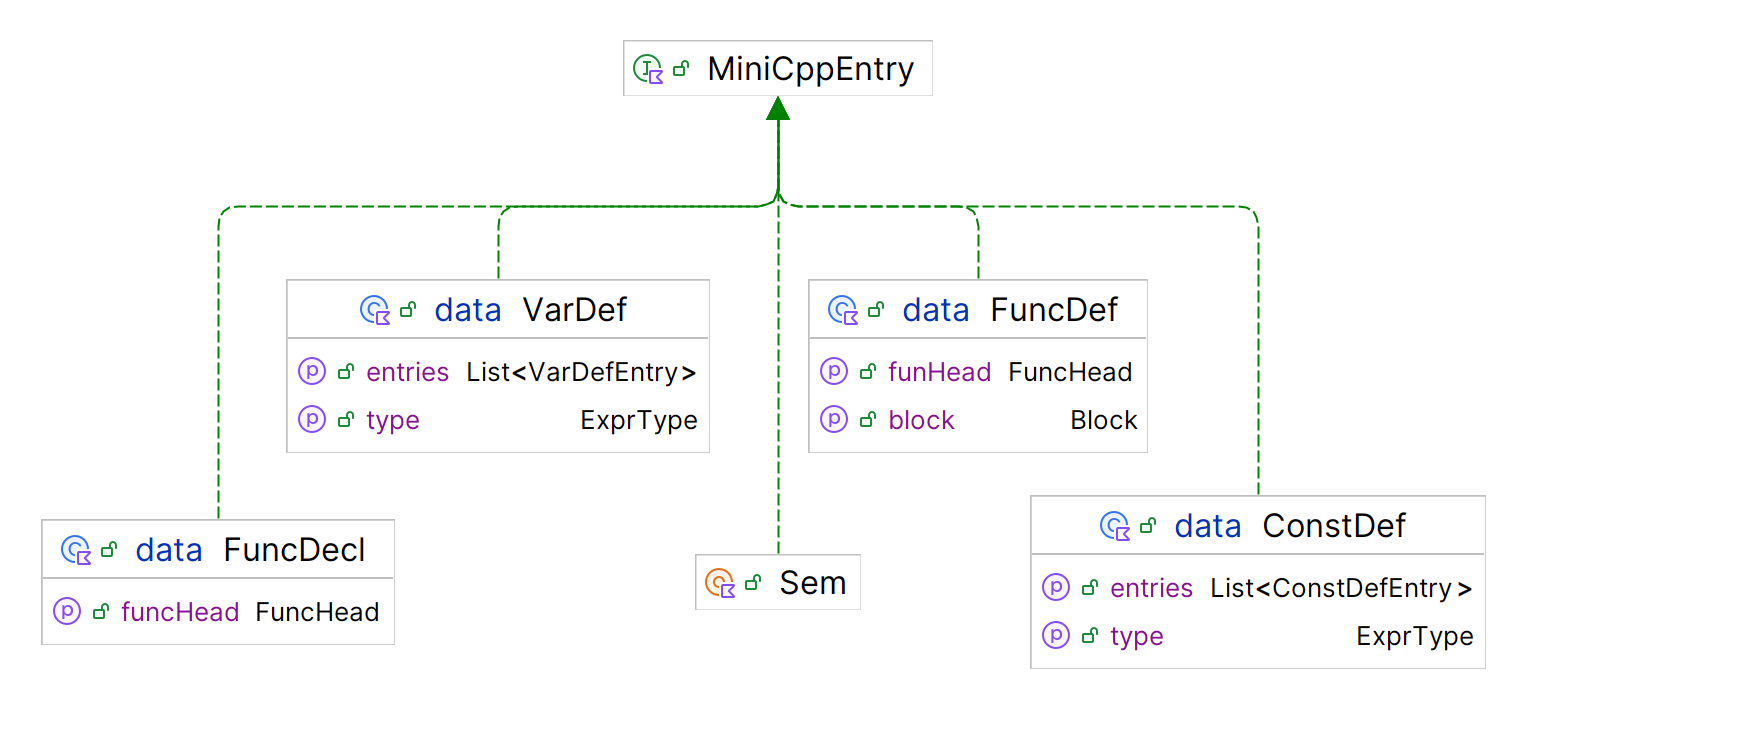
\includegraphics[width=\textwidth]{MiniCppEntries.png}
       \caption{Implementation classes of the \texttt{MiniCppEntry} sealed interface.}
       \label{fig:MiniCppEntriesDiag}
\end{figure}

\begin{KotlinCode}[float,numbers=none,caption=Implementation of the \texttt{ExprType} enum., label=lst:ListExprType]
       enum class ExprType(val descriptor: String = "") {
              VOID("V"),
              BOOL("Z"),
              INT("I"),
              NULLPTR,
              INT_ARR("[I"),
              BOOL_ARR("[Z"),
          }
\end{KotlinCode}

\begin{figure}[]
       \centering
       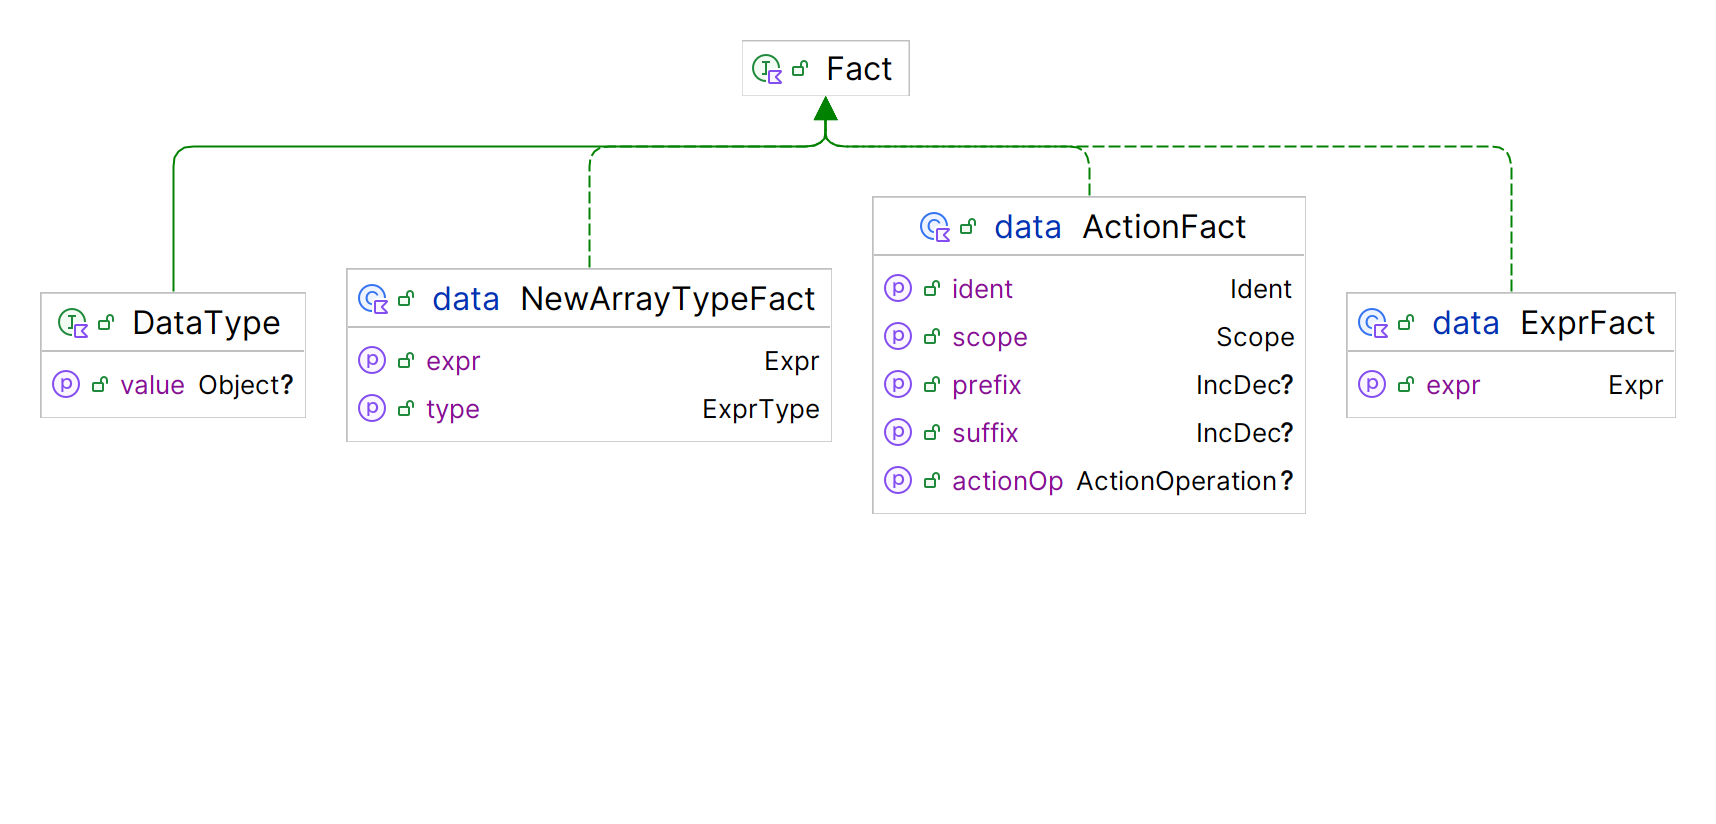
\includegraphics[width=\textwidth]{Fact.png}
       \caption{Implementation classes of the \texttt{Fact} sealed interface.}
       \label{fig:FactDiag}
\end{figure}

%context objects

\section{Symboltable}

Besides the AST a symboltable is needed for the management of the variables and functions of the program. For variables, it is necessary to keep track of their lifetime and shadowing, in case the same variable name is used twice. Since MiniC\verb|++| supports function overloading, each overload of a function needs to be accounted for, so that during the bytecode generation the correct function is called. The \verb|Scope| class is responsible for both variables and functions. It stores information about all variables and functions declared in the current scope. Every time the scope changes, e.g. a function is entered, a new \verb|Scope| instance is created. Each \verb|Scope| instance stores a reference to its parent. This reference is used when a variable or function defined in the parent scope needs to be accessed. Only the root instance does not have a parent scope. In this scope functions and global variables are defined.

\subsection{Variables}

The \verb|Variable| class shown in listing \ref{lst:ScopeVariable} stores information about a variable. The backend uses this information to generate the code for the variable. The identifier is only relevant during the AST generation, as it serves as the link connecting the variable instance to the concrete variable definition node in the AST. The \verb|Variable| class is used for both variable and constant definitions, indicated by the boolean flag \verb|const|. Additionally, for constant values the value itself is also stored in the \verb|constValue| field. In case the variable is defined in the global scope the \verb|static| flag is active. 

Bytecode does not rely on identifiers for stack variables and instead uses indexes. The index of a variable is also stored as a field. The index of a variable is determined during the AST generation. The \verb|getNextAvailableIndex| method returns the next free index for a variable. Listing \ref{lst:ScopeVariableIndex} shows the implementation of the method. Static variables in bytecode use identifiers and therefore are excluded from the index determination process. Indexes start by zero ind are incremented by one. The method determines the current highest index then returns it incremented by one. 


\begin{KotlinCode}[float,numbers=none,caption=Implementation of the \texttt{Variable} class., label=lst:ScopeVariable]
class Variable(
    val ident: Ident,
    val type: ExprType,
    val const: Boolean,
    val static: Boolean,
    var index: Int,
    val constValue: Any? = null
)
\end{KotlinCode}

\begin{KotlinCode}[float,numbers=none,caption=Implementation of the \texttt{getNextAvailableIndex} method., label=lst:ScopeVariableIndex]
private fun getNextAvailableIndex(static: Boolean): Int {
       if (static) return -1
       
       val nonStaticVars = variables.filterNot { it.static }
       return if (nonStaticVars.isEmpty()) {
           parent?.getNextAvailableIndex(static) ?: 0
       } else {
           nonStaticVars.maxOf { it.index } + 1
       }
}
\end{KotlinCode}

\subsection{Function}

Information about a function is managed in the \verb|Function| class shown in listing \ref{lst:ScopeFunction}. A function is identified by its signature: a combination of the identifier and the formal parameter list. MiniC\verb|++| allows the declaration and definition of a function to be specified separately. The \verb|isDefined| flag keeps track of the definition status of a function. This field is further used in a later stage when semantic checks are performed.  


\begin{KotlinCode}[float,numbers=none,caption=Implementation of the \texttt{Function} class., label=lst:ScopeFunction]
data class Function(
       val ident: Ident,
       val returnType: ExprType,
       val formParTypes: List<ExprType>,
       var isDefined: Boolean = false
)
\end{KotlinCode}

\section{Visitor-Implementation}

The visitor-implementation works by traversing the generated syntax tree. When generating the ANTLR combined lexer and parser a visitor interface and base class are generated. The interface \verb|minicppVisitor| is implemented by the \verb|minicppBaseVisitor| base class. This base class contains empty implementations for all \verb|visit| methods of the interface. This allows the developer to only override the methods that are actually needed. The interface is also generic, enabling different return types for the visitor methods based on the specific requirements. 

This implementation creates a concrete visitor class for every type     of the AST. The class extends the \verb|mincCppBaseVisitor| and overrides only the methods relevant for that AST type. The visitor implementation for the \verb|MiniCpp| AST type is shown in listing \ref{lst:VisitorMniCpp}. The AST type serves as the generic type of the base visitor. The \verb|visitMiniCpp| method then returns this type. The input parameter of the method is an instance of the \verb|MiniCppContext| class, which is the syntax tree node representing the \verb|MiniCpp| rule. From this object the relevant information for the AST node is extracted. In this case it contains a list of \verb|miniCppEntry|. Each entry in the list is processed by the \verb|MiniCppEntryVisitor| visitor. The \verb|MiniCppEntryVisitor| overrides all methods for the \verb|varDef|, \verb|funcDecl|, \verb|funcDef| and \verb|SEM| rules. The return type of all methods is the interface \verb|MiniCppEntry|. The root node of the AST is made up of these entries plus the current scope called \verb|globalScope| since it is the parent of all other scopes. The scope instance is passed on to the \verb|MiniCppEntryVisitor| so that for example variable definitions can be added to it.

Named alternatives in the grammar as shown in \ref{lst:ANTLRMiniCppExprBool} for the \verb|termOperator| rule generate the following code seen in listing \ref{lst:VisitorTermOpVis}. The \verb|TermOperatorVisitor| class contains a method for each alternative, eliminating the need to perform not null checks on each symbol to figure out which alternative was produced. Each method returns the enum value corresponding to the node. For more complex rule alternatives as seen in the \verb|callFactEntryOperation| rule, all symbols belonging to an alternative are grouped inside a context object with the same name as the alternative.

The code shown in listing \ref{lst:VisitorExec} produces an AST using the visitor-pattern. The instantiation of the character stream followed by the lexer, token stream and parser is the same for all implementations. The syntax tree is generated by calling the \verb|parser.miniCpp()| method. The syntax tree is then passed into the \verb|visit| method of the \verb|MiniCppVisitor| who initiates the generation of the AST.




\begin{KotlinCode}[float,numbers=none,caption=Implementation of the \texttt{MiniCppVisitor} class., label=lst:VisitorMniCpp]
class MiniCppVisitor(private val className: String) : minicppBaseVisitor<MiniCpp>() 
{
    override fun visitMiniCpp(ctx: minicppParser.MiniCppContext): MiniCpp {
        val scope = Scope(null)
        val entries = ctx.miniCppEntry().map { it.accept(MiniCppEntryVisitor(scope)) }
        return MiniCpp(
            globalScope = scope,
            entries = entries,
            className = className
        )
    }
}
\end{KotlinCode}


\begin{KotlinCode}[float,numbers=none,caption=Implementation of the \texttt{TermOperatorVisitor} class., label=lst:VisitorTermOpVis]
class TermOperatorVisitor : minicppBaseVisitor<TermOperator>() {
    override fun visitStarOperator(ctx: minicppParser.StarOperatorContext): TermOperator {
        return MUL
    }

    override fun visitDivOperator(ctx: minicppParser.DivOperatorContext): TermOperator {
        return DIV
    }

    override fun visitModOperator(ctx: minicppParser.ModOperatorContext): TermOperator {
        return MOD
    }
}
\end{KotlinCode}

\begin{KotlinCode}[float,numbers=none,caption=Code for the generation of the AST using the visitor-pattern., label=lst:VisitorExec]
fun generateASTForFileVisitor(inputStream: InputStream, className: String): MiniCpp 
{
    val charStream = CharStreams.fromStream(inputStream)
    val lexer = minicppLexer(charStream)
    val tokenStream = BufferedTokenStream(lexer)
    val parser = minicppParser(tokenStream)
    return MiniCppVisitor(className).visit(parser.miniCpp())
}
\end{KotlinCode}

\subsection{Listener-Implementation}

The listener-implementation generates the AST during parse process of the syntax tree. Every time a node is entered and exited, listener-methods are called which build up the AST. The listener-implementation follows a similar pattern to the visitor-implementation in that it creates a separate listener for each type of the AST. Similar to the \verb|minicppBaseVisitor| ANTLR also generates a \verb|minicppBaseListener| class. This class contains empty implementations for all listener methods. Only the methods relevant for a specific AST node then need to be overridden. For each node in the syntax tree there is an \verb|enter| and \verb|exit| method, suffixed by the node's name. The \verb|enter| methods also include the context object as an input parameter, however since the node as not been fully parsed yet, no data can be extracted. 

The listener for the \verb|MiniCpp| AST node is shown in listing \ref{lst:ListenerMiniCpp}. The constructor of the \verb|MiniCppListener| requires an instance of the \verb|MiniCppEntryListener|. Via this reference the parsed \verb|miniCppEntry| elements are retrieved. The \verb|exitMiniCpp| method sets the variable \verb|result| which stores the root node of the AST. This variable is used to pass the AST to the rest of program once it has been parsed.

\begin{KotlinCode}[float,numbers=none,caption=Implementation of the \texttt{MiniCppListener} class., label=lst:ListenerMiniCpp]
class MiniCppListener(
    private val entryListener: MiniCppEntryListener,
    private val scopeHandler: ScopeHandler,
    private val className: String
) : minicppBaseListener() {

    lateinit var result: MiniCpp

    override fun exitMiniCpp(ctx: minicppParser.MiniCppContext) {
        result = MiniCpp(className, 
                         scopeHandler.getScope(), 
                         entryListener.getAllEntries()
                         )
    }
}
\end{KotlinCode}

The listeners internally use stacks to store the parsed AST nodes. Listeners that are higher up in the AST hierarchy then fetch the parsed nodes from the respective listeners. The implementation of the \verb|BlockListener| shown in \ref{lst:ListenerBlock} uses the \verb|BlockEntryListener| to get the entries every time a block is exited. The \verb|BlockContext| element knows how many entries it contains and thus the correct number of entries can be retrieved from the block entry stack. This is done via the \verb|getBlockEntry| method, which returns the last parsed block entry and removes it from the stack. The \verb|BlockListener| itself provides the \verb|getBlock| method, which performs the same function for \verb|Block| nodes. Once all entries have been retrieved, their order needs to be reversed. This must be done due to the fact that the entries were retrieved starting with the last parsed entry. By reversing the entries the original program order is preserved. 


\begin{KotlinCode}[float,numbers=none,caption=Implementation of the \texttt{BlockListener} class., label=lst:ListenerBlock]
class BlockListener(private val blockEntryListener: BlockEntryListener,
    private val scopeHandler: ScopeHandler
) : minicppBaseListener() {

    private val blocks = mutableListOf<Block>()
    
    override fun exitBlock(ctx: minicppParser.BlockContext) {
        val scope = scopeHandler.getScope()
        val entries = mutableListOf<BlockEntry>()
        repeat(ctx.blockEntry().size) {
            entries.add(blockEntryListener.getBlockEntry())
        }
        blocks.add(Block(entries = entries.reversed(), scope = scope))
    }
    
    fun getBlock(): Block {
        return blocks.removeLast()
}
}
    \end{KotlinCode}


The code for adding a block entry to the stack is shown in \ref{lst:ListenerBlockEntryExit}. The \verb|BlockEntry| interface is implemented by \verb|Stat|, \verb|VarDef| and \verb|ConstDef|. Even though there are separate listener methods for these types available, the individual nodes need to be retrieved in the \verb|exitBlockEntry| method. There may be statements or variable definitions that are not part of a block and thus, only when a block entry is exited can these nodes be safely retrieved. To retrieve the correct node a null check needs to be performed on all possible productions. 


\begin{KotlinCode}[float,numbers=none,caption=Implementation of the \texttt{exitBlockEntry} method., label=lst:ListenerBlockEntryExit]
    override fun exitBlockEntry(ctx: minicppParser.BlockEntryContext) {
        val entry = when {
            ctx.stat() != null -> statListener.getStat()
            ctx.varDef() != null -> varDefListener.getVarDef()
            ctx.constDef() != null -> constDefListener.getConstDef()
            else -> throw IllegalStateException("Unknown block entry")
        }
        blockEntries.add(entry)
    }
\end{KotlinCode}

For the management of variables and functions the \verb|Scope| class is used, same as in the visitor-based implementation. For the communication between listeners the \verb|ScopeHandler| class is used. The code of this class is shown in listing \ref{lst:ListenerScopeHandler}. Fundamentally, the \verb|ScopeHandler| manages a stack of \verb|Scope| instances. The \verb|init| block instantiates the root scope. The \verb|pushChildScope| method instantiates a new child scope and puts it onto the stack. Whenever a variable or function needs to be added, the current scope can be retrieved via the \verb|getScope| method. The \verb|ScopeHandler| instance is the same over the entire AST generation. All listeners that need to interact with the scope have access to the same instance. 


\begin{KotlinCode}[float,numbers=none,caption=Implementation of the \texttt{ScopeHandler} class., label=lst:ListenerScopeHandler]
class ScopeHandler {

    private val scopes = mutableListOf<Scope>()

    init {
        scopes.add(Scope(null))
    }

    fun getScope(): Scope {
        return scopes.last()
    }

    fun popScope() {
        scopes.removeLast()
    }

    fun pushChildScope() {
        scopes.add(Scope(getScope()))
    }
}
\end{KotlinCode}

The execution process is similar to the visitor-implementation shown in listing \ref{lst:VisitorExec}. First all the listener instances are created. Depending on the listener it's constructor may contain one or more references to other listeners from where AST nodes can be retrieved. In some cases the relation between the listeners is too complex to be able to pass all the required listeners as constructor parameters. For such cases a separate \verb|initialize| method is used which supplies the required listeners. The \verb|minicppParser| then provides a method to register listeners. Every listener is registered to the parser using this method. The \verb|miniCpp| method of the parser then starts the parsing process. Once this method has finished executing, the generated AST can be retrieved from the \verb|result| variable of the \verb|MiniCppListener|.

\section{ATG-Implementation}

The implementation of the attributed grammar (ATG) is an extension of the grammar shown in \ref{cha:ANTLRGrammar}. As ANTLR does not support Kotlin as an implementation language, the ATG is implemented in Java. The code written in the grammar file is directly embedded into the generated parser and executed during the parse process. Because Java and Kotlin are compatible on a bytecode level, the AST which is written in Kotlin, can be used in the Java based ATG implementation. 

Since the AST and other needed classes like \verb|ArrayList| are in different packages, they need to be imported. For this the \verb|@header| section is used. The code written in this section is added to the top of the generated parser before the class declaration and thus can be used for the required import statements. 

Similar to the listener-implementation, the ATG-implementation relies on stacks for the management of AST nodes. The stacks are defined in the \verb|members| section. This section is pasted into the class body of the parser, and thus member variables can be defined here. Besides the stacks, also the result of the AST generation, the \verb|MiniCpp| object is stored as an instance variable. The scope handling is performed in the same way as in the listener-implementation via the \verb|ScopeHandler| class. Some utility methods are also defined in the member section. 


Listing \ref{lst:ANTLRATGMiniCpp} shows the ATG for the \verb|miniCpp| and \verb|miniCppEntry| rules. The semantic action for the \verb|miniCpp| rule instantiates the \verb|MiniCpp| AST class with the current scope and all \verb|miniCppEntries|. The positioning of the semantic action after the \verb|EOF| causes it to be executed at the end of the parsing process after all \verb|miniCppEntry| nodes have been parsed. The semantic actions for the \verb|miniCppEntry| rule retrieve nodes from their respective stack and put it onto the \verb|miniCppEntries| stack.   

\begin{AntlrCode}[float,numbers=none,caption=ATG for the \texttt{miniCpp} and \texttt{miniCppEntry} rules., label=lst:ANTLRATGMiniCpp]
    miniCpp: (miniCppEntry)* EOF                    
    { result = new MiniCpp(className, scopeHandler.getScope(), miniCppEntries.stream().toList()); }
    ;
miniCppEntry:     
      constDef                  { miniCppEntries.push(constDefs.pop()); }
    | varDef                    { miniCppEntries.push(varDefs.pop()); }
    | funcDecl                  { miniCppEntries.push(funcDecls.pop()); }
    | funcDef                   { miniCppEntries.push(funcDefs.pop()); }
    | SEM                       { miniCppEntries.push(Sem.INSTANCE); }
;
\end{AntlrCode}
    

In the case of rules like \verb|constDef| where there are one or more \verb|constDefEntry| nodes stored inside the \verb|ConstDef| AST node, a list is used to store the entries during the parse of the rule. This process is shown in listing \ref{lst:ANTLRATGConstDef}. After the first \verb|constDefEntry| is parsed, a list is created which stores all following \verb|constDefEntry| nodes.
At the end of the rule a new \verb|ConstDef| node containing all \verb|constDefEntry| nodes, is instantiated and put onto the \verb|constDefs| stack.



\begin{AntlrCode}[float,numbers=none,caption=ATG for the \texttt{constDef} rule., label=lst:ANTLRATGConstDef]
constDef:    
    CONST type constDefEntry          
        { var entries = new ArrayList(List.of(constDefEntries.pop())); }
    (
        ',' constDefEntry           
        { entries.add(constDefEntries.pop());}
    ) 
    * SEM
        { constDefs.push(new ConstDef(types.pop(), entries)); }
\end{AntlrCode}


The ATG code visible in listing \ref{lst:ANTLRATGInit}, shows the rules \verb|init| and \verb|initOption|. For the \verb|BooleanInit| and \verb|IntInit| alternatives, values of their respective terminal classes must be processed. For the \verb|BooleanInit| alternative this means reading the text of the terminal class and parsing it to a boolean. The \verb|NullptrInit| alternative just puts the singleton instance of the \verb|NullPtrType| on the stack and thus does not need to read any value. For the \verb|IntInit| alternative, the integer value is retrieved by parsing the text of the \verb|INT| terminal class. In case a sign is present it is checked if it is negative. In case of a negative sign the integer value is inverted. 

\begin{AntlrCode}[float,numbers=none,caption=ATG for the \texttt{initOption} rule., label=lst:ANTLRATGInit]
init:        '='  initOption;
initOption:    
   BOOLEAN                          
       { inits.push(new Init(newBoolType(
            Boolean.parseBoolean($BOOLEAN.text)
          )));  
       }             #BooleanInit
 | NULLPTR                          
       { inits.push(new Init(NullPtrType.INSTANCE)); }                                     #NullptrInit
 | (SIGN)? INT
       {
         var value = Integer.parseInt($INT.text);
         if ($SIGN != null && $SIGN.text.equals("-")) {
             value = -value;
         }
         inits.push(new Init(new IntType(value)));
       }             #IntInit
;
    \end{AntlrCode}


The execution of the ATG functions in the same way as for the visitor-implementation in listing \ref{lst:VisitorExec}. The parser is executed by calling the \verb|miniCpp| method. Once this method has finished executing, the generated AST can be retrieved via the \verb|result| variable of the parser. 




